% Chapter 7

\chapter{Bayesian Optimization Of A Hybrid System For Robust Ocean Wave Features Prediction} % Write in your own chapter title
\label{Chapter7}
\lhead{Chapter \ref{Chapter7}. 
\emph{Bayesian Optimization Of A Hybrid System For Robust Ocean Wave Features Prediction}} % Write in your own chapter title to set the page header

{\bf \small{
This chapter describes a Bayesian optimization application on a real case involving the robust prediction of ocean wave features. Specifically, we propose the Bayesian optimization of a hybrid Grouping Genetic Algorithm with an Extreme Learning Machine (GGA-ELM) approach. The system uses data from neighbor stations (usually buoys) in order to predict the significant wave height and the wave energy flux at a goal marine structure facility. The proposed BO methodology has been tested in a real problem involving buoys data in the Western coast of the USA. The results show that BO outperforms the performance of a random search of the hyper-parameters space and the result given by a human expert on the problem.
}}

\section{Introduction}
The accurate prediction of waves features plays a key role in different ocean engineering--related activities, such as safe ship navigation \citep{zheng2016path,liu2016path}, the design of marine structures \citep{comola2014damage,kim2014determining}, such as oil platforms and harbours, and in marine energy management problems \cite{arinaga2012atlas,esteban2012current}, like the proper operation of wave energy converters \citep{lopez2013review}, among others. Thus, the topic has a clear impact on human safety, economics and clean energy production. One of the most important features to define the severity of a given ocean wave field is the significant wave height, $H_{m_0}$. $H_{m_0}$ is usually estimated using in-situ sensors, such as buoys, recording time series of wave elevation information. Buoys provide reliable sea state information that characterizes wave field in a fixed position (i.e. the mooring point). In addition, as buoys are anchored in a hostile media (the ocean), the probability that measuring problems (and therefore missing data) occur in situations of severe weather is very high \citep{rao2005hindcasting}. Besides this, marine energy is currently one of the most promising sources of renewable energy, still minor at a global level, but playing a major role in several offshore islands \citep{bahaj2011generating,antonio2010wave,fadaeenejad2014new,rusu2012wave}. In this case, the accurate estimation of the wave energy flux $P$ is relevant to characterize the wave energy production from Wave Energy Converters (WECs) facilities \citep{cuadra2016computational}.

In this chapter we test a BO methodology to improve the performance of a hybrid prediction system for wave features ($H_{m_0}$ and $P$) prediction. Specifically, the prediction system is formed by a Grouping Genetic Algorithm for feature selection, and an Extreme Learning Machine for carrying out the final energy flux prediction \citep{cornejo2016significant}. This hybrid prediction system has a number of parameters that may affect its final performance, and need to be previously specified by the practitioner. Traditionally, these parameters have been manually tuned by a human expert, with experience in both the algorithm and the problem domain. However, it is possible to obtain better results by an automatic fine tuning of the prediction system's parameters. In this case, the parameters of GGA-ELM approach include the probability of mutation in the GGA or the number of neurons in the ELM hidden layer, among others. We propose then to use a Bayesian Optimization (BO) approach to automatically optimize the parameters of the whole prediction system (GGA-ELM), with the aim of improving its performance in wave energy prediction problems. BO has been shown to obtain good results in the task of obtaining good parameter values for prediction systems \citep{snoek2012practical}. In the chapter we detail the basic prediction system considered and the BO methodology implemented, along with the improvements obtained in real problems of $H_{m_0}$ and $P$ prediction in the Western coast of the USA.

The rest of the chapter is organized as follows: the next section details the calculation of the features of interest in ocean wave characterization, $H_{m_0}$ and $P$ in this case. Section \ref{sec:hybrid_system} describes the main characteristics of the hybrid system to be optimized, which is formed by a GGA and an ELM for prediction. Section \ref{sec:Experiments} presents the real experiments that deal with buoys in the Western coast of the USA whose results show how BO outperforms the random search of the space and the human expert criterion. Finally, Section \ref{sec:Conclusions} closes the chapter with conclusions and remarks on this research.

\section{Wave Features of Interest: Calculation of $H_{m_0}$ and $P$}\label{sec:hybrid_system}
In the evaluation of marine systems it is essential to previously characterize as accurately as possible the wave features of the zone under study. For example, in a wave energy facility, it is necessary to characterize the amount of wave energy available at a particular location, which is given by features such as $H_{m_0}$ and $P$. In order to obtain these features, it is necessary to focus on the water surface, and within the framework of the linear wave theory, the vertical wave elevation, $\eta(\mathbf{r},t)$, at a point $\mathbf{r}=(x,y)$ on the sea surface at time $t$ can be assumed as a superposition of different monochromatic wave components \citep{borge2013detection,yoshimi2010random}. This model is appropriate when the free wave components do not vary appreciably in space and time (that is, statistical temporal stationarity and spatial homogeneity can be assumed \citep{yoshimi2010random}).

In the model described, the concept of ``sea state'' refers to the sea area and the time interval in which the statistical and spectral characteristics of the wave do not change considerably (statistical temporal stationarity and spatial homogeneity). The features of a given sea state are then the combined contribution of all features from different sources. For example, the ``wind sea'' occurs when the waves are caused by the energy transferred between the local wind and the free surface of the sea. The ``swell'' is the situation in which the waves have been generated by winds blowing on another far area (for instance, by storms), and propagate towards the region of observation. Usually, sea states are the composition of these two pure states, forming multi-modal or mixed seas.
In a given sea state, the wave elevation $\eta(\mathbf{r},t)$ with respect to the mean ocean level can be assumed as a zero-mean Gaussian \emph{stochastic process}, with statistical symmetry between wave maxima and minima. A buoy deployed at point $\mathbf{r}_B$ can take samples of this process, $\eta(\mathbf{r}_B,t_j)$ $j=1,2, \cdots , t_{\mathrm{MAX}}$, generating thus a time series of empirical vertical wave elevations. The Discrete Fourier Transform (DFT) of this sequence, using the Fast Fourier Transform (FFT) algorithm, allows for estimating the \emph{spectral density} $S(f)$. Its spectral moments of order $n$ can be computed as follows:

\begin{equation}\label{equation_Spectral_Moments}
 m_n = \int_{0} ^{\infty} f^n S(f) df.
\end{equation}

The Significant Wave Height (SWH) is defined as the average (in meters) of the highest one-third of all the wave heights during a 20-minute sampling period, and it has been widely studied.
It can be calculated from the moment of order $0$ in Equation (\ref{equation_Spectral_Moments}), as follows:

\begin{equation}
H_{m_0} = 4 \cdot (m_0)^{1/2}\,.
\end{equation}

On the other hand, the wave energy flux is a first indicator of the amount of wave energy available in a given area of the ocean. Wave energy flux $P$, or power density per meter of wave crest can be computed as

\begin{equation} \label{eq_P_Hs_Te}
 P =  \frac{\rho g^2}{4 \pi}\int_{0}^{\infty}\frac{S(f)}{f}  df  =   \frac{\rho g^2}{4 \pi}   m_{-1} =   \frac{\rho g^2}{64 \pi}   H_{m_0}^2  \cdot T_e,
\end{equation}
where $\rho$ is the sea water density (1025 kg/m$^3$), $g$ is the acceleration due to gravity, $H_{m_0} = 4  \sqrt{m_0}$ is the spectral estimation of the significant wave height, and $T_e \equiv T_{-1,0} = m_{-1} / m_0$ is an estimation of the mean wave period, normally known as the period of energy, which is used in the design of turbines for wave energy conversion \citep{cahill2013wave}. Expression (\ref{eq_P_Hs_Te}) (with $H_{m_0}$ in meters and $T_e$ in seconds) leads to

\begin{equation}
P =  0.49 \cdot   H_{m_0}^2 \cdot T_e,
\end{equation}
measured in $kW/m$, which helps engineers estimate the amount of wave energy available when planning the deployment of WECs at a given location.
The grouping genetic algorithm (GGA) is a type of evolutionary algorithm especially suited to tackle grouping problems, i.e., problems where a number of items must be assigned to a set of predefined groups \citep{falkenauer1993grouping,falkenauer1998genetic}. The GGA has shown very good performance on different real applications and problems \citep{agustin2011near,agustin2009hybrid,brown2005evaluating,james2007hybrid,james2007hybridb,de2000grouping}. In the GGA, the encoding, crossover and mutation operators of traditional GAs are modified to better deal with grouping problems. In this chapter we use the GGA to obtain a reduced set of features (feature selection) in a context of $H_{m_0}$ and $P$ prediction. We structure the description of the GGA in Encoding, Operators and Fitness Function calculation (Extreme Learning Machine).

\subsection{Problem Encoding}\label{encoding}

The GGA is a variable-length genetic algorithm. The encoding is defined by separating each individual in the algorithm into two parts: an {\em assignment} part, which associates each item to a given group, and a {\em group} part, which defines the groups that must be taken into account for the individual. In problems where the number of groups is not previously defined, it is straightforward that this is a variable-length algorithm: the group part varies from one individual to another. In our implementation of the GGA for feature selection, an individual ${\bf c}$ has the form ${\bf c}=[{\bf a}|{\bf g}]$. An example of an individual in the proposed GGA for a feature selection problem, with 20 features and 4 groups, is the following:

1 1 2 3 1 4 1 4 3 4 4 1 2 4 4 2 3 1 3 2 $|$ 1 2 3 4

where the group 1 includes features $\{1,2,5,7,12,18\}$, group 2 features $\{3,13,16,20\}$, group 3 features \{4,9,17,19\} and finally group 4 includes features $\{6,8,10,11,14,15\}$.

\subsection{Genetic Operators}

In this chapter we use a tournament-based selection mechanism \citep{yao1999evolutionary}. This mechanism has been shown to be one of the most effective selection operators, avoiding super-individuals and performing a excellent exploration of the search space. Regarding the crossover operator, we have chosen a modified version of the one initially proposed by \cite{falkenauer1993grouping,falkenauer1998genetic}. It follows the process outlined in Figure \ref{cruce_GGA}:

\begin{itemize}
\item[1.] Choose two parents from the current population, at random.
\item[2.] Randomly select two points for the crossover, from the ``Groups'' part of parent 1, then, all the groups between the two cross-points are selected. In the example of Figure \ref{cruce_GGA} the two crossover points are $G_1$ and $G_2$. Note that, in this case the items of parent1 belonging to group $G_{1}$ and $G_{2}$ are 1, 2, 4, 5, and 6.
\item[3.] Insert the selected section of the ``Groups'' part into the second parent. After the insertion in the example of Figure \ref{cruce_GGA}, the assignment of the nodes 1, 2, 4, 5 and 6 of the offspring individual will be those of parent 1, while the rest of the nodes' assignment are those of parent 2. The ``Groups'' part of the offspring individual is that of parent 2 plus the selected section of parent 1 (8 groups in total, in this case).
\item[4.] Modify the ``Groups'' part of the offspring individual with their corresponding number. In the example, $G$ = 1 \hspace{1mm} 2 \hspace{1mm} 3 \hspace{1mm} 4 \hspace{1mm} 5 \hspace{1mm} 6 \hspace{1mm} 1 \hspace{1mm} 2 is modified into $G$ = 1 \hspace{1mm} 2 \hspace{1mm} 3 \hspace{1mm} 4 \hspace{1mm} 5 \hspace{1mm} 6 \hspace{1mm} 7 \hspace{1mm} 8. Modify also the assignment part accordingly.
\item[5.] Remove any empty groups in the offspring individual. In the example considered, it is found that groups 1, 2, 3, and 6 are empty, so we can eliminate these groups' identification number and rearrange the rest. The final offspring is then obtained.
\end{itemize}

\begin{figure}[b]
\centering
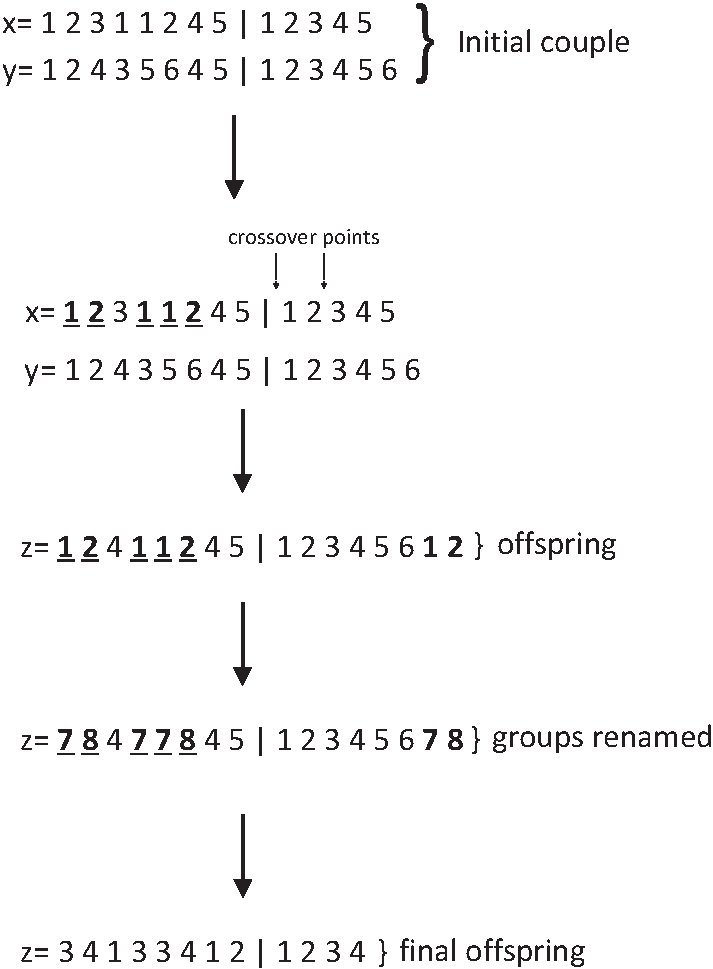
\includegraphics[width=0.75\textwidth]{Figures/cruce_GGA.pdf} \\
\caption{\label{cruce_GGA} Outline of the grouping crossover implemented in the proposed GGA.}
\end{figure}

Regarding mutation operator, we apply a swapping mutation in which two items are interchanged (swapping this way the assignment of features to different groups). This procedure is carried out with a very low probability ($P_m=0.01$), to avoid increasing of the random search in the process. In the next section we describe the fitness function used to guide the search in the GGA, the ELM neural network, which is a very fast algorithm with excellent performance in prediction problems.

\subsection{Fitness Function: the Extreme Learning Machine}
An ELM is a fast learning method based on the structure of MLPs with a novel way of training feed-forward neural networks \citep{huang2006extreme}. One of the most important characteristics of the ELM training is the randomness in the process where the network weights are set, obtaining, in this way, a pseudo-inverse of the hidden-layer output matrix. The simplicity of this technique makes the training algorithm extremely fast. Moreover, it is remarkable the outstanding performance shown when compared to other learning methods. For example, it is usually better than other established approaches such as classical MLPs or SVRs.

The ELM algorithm can be explained as follows: given a training set $$\mathbb{T} = {(\mathbf{x}_i,\boldsymbol{W}_i) | \mathbf{x}_i \in \mathbb{R}^n, \boldsymbol{W}_i \in \mathbb{R}, i=1, \cdots, l}$$, an activation function $g(x)$ and number of hidden nodes ($\tilde{N}$),

\begin{enumerate}
        \item Randomly assign inputs weights $\mathbf{w}_i$ and bias $b_i$, $i = 1, \cdots ,\tilde{N}$.
        \item Calculate the hidden layer output matrix $\mathbf{H}$, defined as

        \begin{equation}
        \mathbf{H} = \left [ \begin{array}{ccc}
        g( \mathbf{w}_1 \mathbf{x}_1 + b_1) & \cdots & g(\mathbf{w}_{\tilde{N}} \mathbf{x}_1 + b_{\tilde{N}}) \\
        \vdots & \cdots & \vdots \\
        g(\mathbf{w}_1 \mathbf{x}_l + b_1) & \cdots & g(\mathbf{w}_{\tilde{N}} \mathbf{x}_N + b_{\tilde{N}})
        \end{array}
        \right ]_{l \times \tilde{N}}
        \end{equation}


        \item Calculate the output weight vector $\beta$ as
        \begin{equation}
        \beta = \mathbf{H}^\dagger \mathbf{T},
        \end{equation}
        where $\mathbf{H}^\dagger$ stands for the Moore-Penrose inverse of matrix $\mathbf{H}$ \citep{huang2006extreme}, and $\mathbf{T}$ is the training output vector, $\mathbf{T}=[\boldsymbol{W}_1,\cdots,\boldsymbol{W}_l]^T$.
\end{enumerate}

The number of hidden nodes ($\tilde{N}$) is a free parameter of the ELM training, and it can be fixed initially, or in a best convenient way, it must be estimated for obtaining good results as a part of a validation set in the learning process. Hence, scanning a range of $\tilde{N}$ values is the solution for this problem.

These experiments use the Matlab ELM implementation by G. B. Huang, freely available on the Internet (\url{http://www.ntu.edu.sg/home/egbhuang/elm\_codes.html}).

\section{Experiments}\label{sec:Experiments}
This section presents the experiments carried out in order to show the improvement of performance in the system when it is optimized with the BO techniques shown above. We consider a real problem of wave energy flux prediction ($P =  0.49\cdot   H_s^2 \cdot T_e$ kW/m) from marine buoys \citep{yoshimi2010random}. Figure \ref{boyas_con_b} shows the three buoys considered in this study at the Western coast of the USA, whose data bases are obtained from the National Data Buoy Center. The objective of the problem is to carry out the reconstruction of buoy 46069 from a number of predictive variables from the other two buoys. Thus, 10 predictive variables measured at each neighbor buoy are considered (a total of 20 predictive variables to carry out the reconstruction). Table \ref{tab:databaseSets} shows details of the predictive variables for this problem. Data for two complete years (1st January 2009 to 31st December 2010) are used, since complete data (without missing values in predictive and objective $P$) are available for that period in the three buoys. These data are divided into training set (year 2009) and test set (year 2010) to evaluate the performance of the proposed algorithm.

\begin{figure}[htbp]
\centering
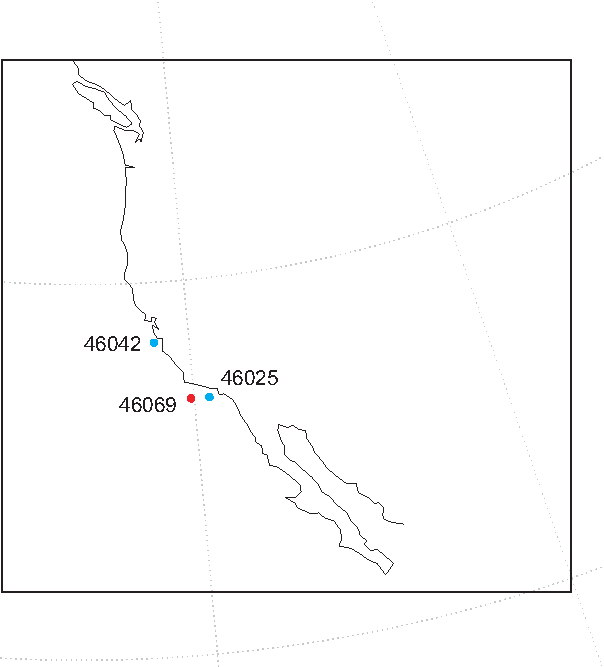
\includegraphics[width=0.7\textwidth]{Figures/alcala/Mapa_boyas_con_b_California.pdf} \\
\caption{\label{boyas_con_b} Western USA Buoys considered in this study. In red buoy where the $P$ prediction is carried out from data at blue ones.}
\end{figure}

\begin{table}[htbp]
\begin{center}
\caption{Predictive variables used in the experiments.}
\vspace{0.3cm}
\label{tab:databaseSets}
\begin{tabular}{ccc}
       \hline
Acronym & Predictive            & units \\
&variable&\\
\hline
\hline
WDIR\         & Wind direction\            & [degrees]\\
WSPD\         & Wind speed\                & [m/s]\\
GST\          & Gust speed\                & [m/s]\\
WVHT\         & Significant wave height\   &  [m]\\
DPD\          & Dominant wave period\      & [sec]\\
APD\          & Average period\            & [sec]\\
MWD\          & Direction DPD\             & [degrees]\\
PRES\         & Atmospheric pressure\      & [hPa]\\
ATMP\         & Air temperature\           & [Celsius]\\
WTMP\         & water temperature\         & [Celsius]\\
\hline
\end{tabular}
\end{center}
\end{table}

We evaluate the utility of the BO techniques for finding good parameters for the prediction system described in Section \ref{sec:hybrid_system}. More precisely, we try to find the parameters that minimize the RMSE of the best individual found by the GGA on a
validation set that contains $33\%$ of the total data available. The parameters of the GGA that are adjusted are
the probability of mutation $p\in [0, 0.3]$, the percentage of confrontation in the tournament
$q\in[0.5,1.0]$, and the number of epochs $e\in [50, 200]$. On the other hand, the parameters of the
ELM that is used to evaluate the fitness in the GGA are also adjusted. These parameters are the number of hidden units
$n\in[50,150]$ and the logarithm of the regularization constant of a ridge regression
estimator, that is used to find the weights of the output layer $\gamma \in [-15,-3]$.
Note that a ridge regression estimator for the output layer weights allows for a more flexible
model than the standard ELM, as the standard ELM is retrieved when $\gamma$ is
negative and large \citep{albert1972regression}.

We compare the BO method with two techniques. The first technique is a random exploration of
the space of parameters. The second technique is a configuration specified by a human
expert. Namely, $p=0.02$, $q=0.8$, $e=200$, $n=150$ and $\gamma = -10$. These are reasonable
values that are expected to perform well in the specific application tackled. We set our computational budget to $50$ different
parameter evaluations for both the BO and the random exploration strategy. After each
evaluation, we report the performance of the best solution found. The experiments are repeated
for $50$ different random seeds and we report average results. All BO experiments are carried out
using the acquisition function EI and the software for BO Spearmint.

Fig. \ref{bo:experiments} and \ref{bo:hexperiments} show the average results obtained and the corresponding error bars for the
Wave Energy Flux and the Wave Height optimization. This figure shows the average RMSE of each method (BO and random exploration) on the validation
set as a function of the number of configurations evaluated. The performance of the configuration
specified by a human expert is also shown. We observe that the BO strategy performs best.
After a few evaluations is able to outperform the results of the human expert
and it provides results that are similar or better than the ones obtained by the random
exploration strategy with a smaller number of evaluations.
\begin{figure}[!htb]
\centering
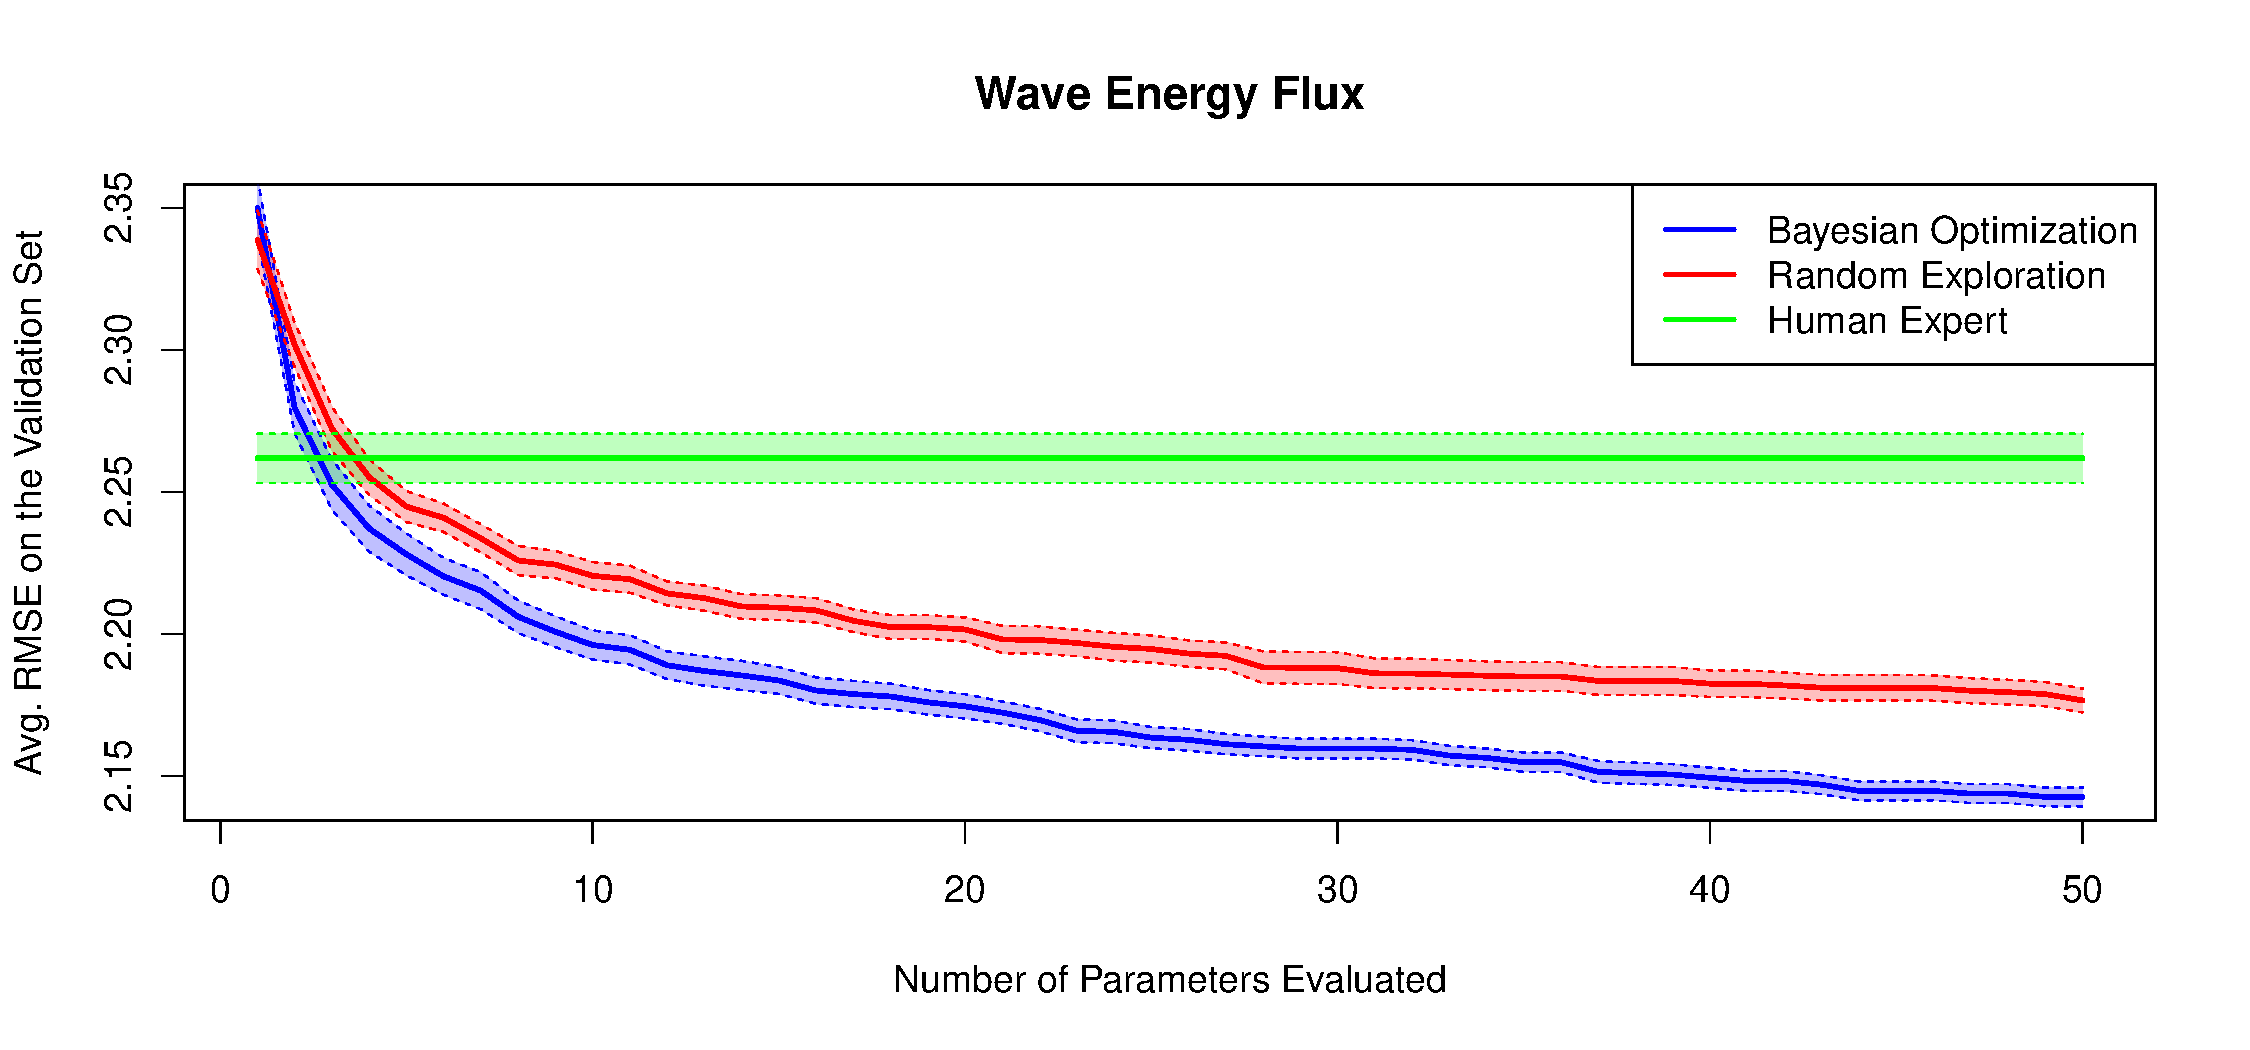
\includegraphics[width=0.8\textwidth]{Figures/alcala/bo.pdf}
\caption{\label{bo:experiments}
        Average results obtained for the Wave Energy Flux optimization
        after evaluating the performance of 50 different parameters for
        the BO technique and a random exploration of the parameter space. The performance a
        configuration specified by a human expert is also shown for comparison.
}
\end{figure}
\begin{figure}[!htb]
\centering
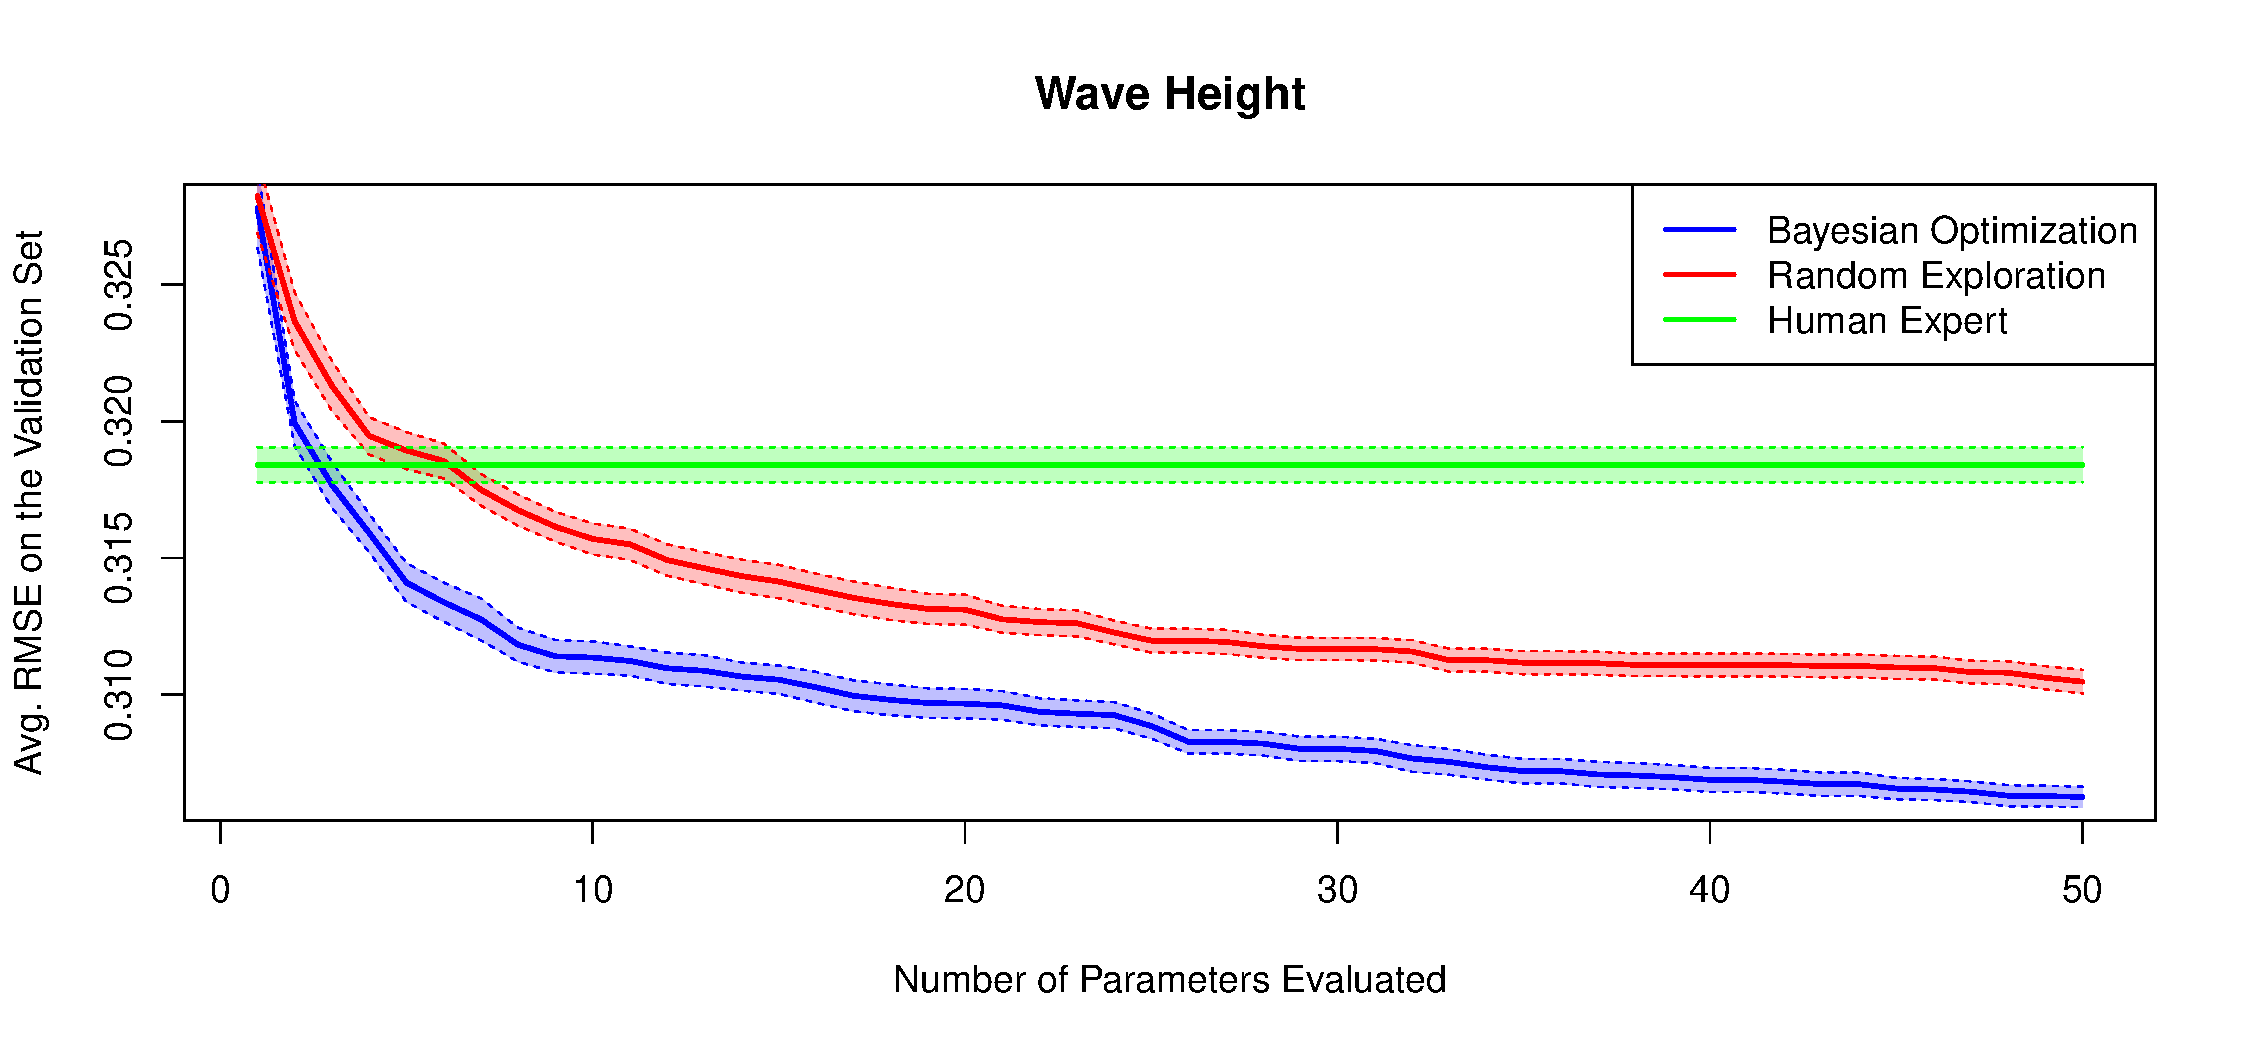
\includegraphics[width=0.8\textwidth]{Figures/alcala/bo_height.pdf}
\caption{\label{bo:hexperiments}
        Wave Height optimization average results of the performance of the 50 different parameter values
        selected by the BO technique and a random exploration of the parameter space.
        The plot also shows the performance of the parameter values selected by a human expert.
}
\end{figure}

\section{Conclusions}\label{sec:Conclusions}
In this section we have shown how a hybrid prediction system for wave energy prediction can be improved by means of BO. The prediction system is formed by a grouping genetic algorithm for feature selection, and an Extreme Learning Machine for effective prediction of the target variable, the wave energy flux in this case. After this feature selection process, the final prediction of the wave energy flux is obtained by means of an ELM or a SVR approach.
The chapter describes the specific application of BO in the optimization of the GGA-ELM for a real problem of wave energy flux prediction from buoys data in Western California USA. The results show how BO outperforms the results given by a random search of the space and the results given by the criterion of a human expert on the problem. 
